\section{Quantum Gates and Magic}
\begin{example}
Set $\{AND, OR, NOT\}$ is universal for classical computation, i.e., it can be used
to compute arbitrary classical function. 
\end{example} 

Here: 3 universality constructions. Result: any unitary operation can be approximated to an arbitrary accuracy using $H$, $CNOT$ and $\frac{\pi}{8}$ gates. \\
Originally, the phase gate P used to be included in the construction, since it is important for the fault-tolerant cases. \\
Reminder: $P$ gate can be constructed from two $\frac{\pi}{8}$ gates. \\

\section{Step 1}
{In the first stage of the construction, we restrict ourselves to working with the matrix form of unitary operations. \\
\begin{claim}
    Let $U$ be a unitary matrix on a d-dimensional Hilbert space. Then: $U$ can be decomposed exactly into a product of 2-level unitary matrices.
\end{claim}
Instead of providing a general proof, we will instead look at $U$ being a $3 \times 3$ matrix, and figure out the decomposition explicitly.\\
\begin{example}
    ($3 \times 3$ case): Consider
    \begin{center}
        $U = 
        \begin{bmatrix}
            a & d & g  \\
            b & e & h  \\
            c & f & j  \\
        \end{bmatrix} $.
    \end{center}
     We want to find $U_1, U_2, U_3$, such that $U_3U_2U_1U = \mathds{1}$, i.e., $U^\dagger_1U^\dagger_2U^\dagger_3=U$.
\end{example}
Note: $U_j$ are $2$-level unitary matrices $\forall j=1,2,3$, therefore, so are the ${U_j}^\dagger$. \\
\begin{proof} \\
If $b=0 \Rightarrow$ 
\begin{center}
set $U_1 :=
\begin{bmatrix}
    1 & 0 & 0  \\
    0 & 1 & 0  \\
    0 & 0 & 1  \\
\end{bmatrix} $.
\end{center}
If $b \neq 0 \Rightarrow$ 
\begin{center}
set $U_1 :=
\begin{bmatrix}
    \frac{a^*}{\sqrt{{\abs a}^2 + {\abs b}^2}} & \frac{b^*}{\sqrt{{\abs a}^2 + {\abs b}^2}} & 0  \\
    \frac{b}{\sqrt{{\abs a}^2 + {\abs b}^2}} & \frac{-a}{\sqrt{{\abs a}^2 + {\abs b}^2}} & 0  \\
    0 & 0 & 1  \\
\end{bmatrix} $.
\end{center}
What we arrive at, in any of the above cases, is a 2-level unitary matrix (can be easily verified by calculating). Moreover: \\
\begin{center}
    $U_1U = \begin{bmatrix}
    a^\prime & d^\prime & g^\prime  \\
    0 & e^\prime & h^\prime  \\
    c^\prime & f^\prime & j^\prime  \\
\end{bmatrix} $.
\end{center}
Next: want to get rid of the value in the bottom left corner $\Rightarrow$ proceed analogously: \\
\begin{itemize}
    \item $c=0 \Rightarrow$ set 
        \begin{center}
        $U_2 :=
            \begin{bmatrix}
            {a^\prime}^* & 0 & 0  \\
            0 & 1 & 0  \\
            0 & 0 & 1  \\
            \end{bmatrix}$.
        \end{center}
        
    \item $c \neq 0 \Rightarrow$ set 
        \begin{center}
            $U_2 :=
        \begin{bmatrix}
            * & 0 & *  \\
            0 & 1 & 0  \\
            * & 0 & *  \\
        \end{bmatrix} $,
        \end{center}
        where $*$'s denote similar fractions, involving square roots, as in the case of $U_1$.
\end{itemize}
Once again, we get a 2-level unitary matrix $U_2$ that satisfies 
\begin{center}
    $U_2U_1U=
\begin{bmatrix}
    1 & d^{\prime\prime} & g^{\prime\prime}  \\
    0 & e^{\prime\prime} & h^{\prime\prime}  \\
    0 & f^{\prime\prime} & j^{\prime\prime}  \\
\end{bmatrix}$.
\end{center} 
\\

Important consequence, used to simplify the proof: \\
$U, U_1, U_2$ are unitary $\Rightarrow$ $U_2U_1U$ is unitary $\Rightarrow$ $d'' = g'' = 0$ (for the norm of the first line of the matrix to be 1).\\

Lastly, set 
\begin{center}
$U_3 := 
\begin{bmatrix}
    1 & 0 & 0  \\
    0 & {e^{\prime\prime}}^* & {h^{\prime\prime}}^*  \\
    0 & {f^{\prime\prime}}^* & {j^{\prime\prime}}^*  \\
\end{bmatrix}$
\end{center}
to obtain: 
    $U_3U_2U_1U= \mathds{1}$.     
\end{proof}

On generalization: if $U$ is a matrix on a $d$-dimensional space, then we need to find matrices $U_1, \cdots, U_{d-1}$ such that: \\
\begin{center}
    $U_{d-1} \cdots U_1U = M $,
\end{center}
where $M$ has $1$ in the top left corner, $0$'s in the rest of the first column and first row, and some matrix $A$ of dimension $d-1$.
Then, repeat the procedure for the internal matrix $A$, and so on. \\

End result: $U=V_1 \cdots V_k$ and $k \leq d*(d-1)/2$. The bound comes from the fact that we need $d$ matrices to get a unitary matrix of size $(d-1) \times (d-1)$, $(d-1)$ matrices to get to the $(d-2) \times (d-2)$ matrix, similar for next steps.
}
\section{Step 2}
{Next step: expressing 2-level unitaries, using only single-qubit operations and CNOTs. \\
\begin{claim}
    Arbitrary 2-level unitary operation on $n$ qubits can be implemented, using only single-qubit and CNOT gates.
\end{claim} 
Here, we will take a look at an example, in order to illustrate the procedure. Further details can be found in the Nielsen-Chuang textbook, Chapter 4.5.2. \\
\begin{example}
    3 qubits ($8 \times 8$ matrix):
\end{example}
Assume, we have a 2-level unitary 
\begin{center}
   $U = 
\begin{bmatrix}
 a & 0 & 0 & 0 & 0 & 0 & 0 & c \\
 0 & 1 & 0 & 0 & 0 & 0 & 0 & 0 \\    
 0 & 0 & 1 & 0 & 0 & 0 & 0 & 0 \\
 0 & 0 & 0 & 1 & 0 & 0 & 0 & 0 \\
 0 & 0 & 0 & 0 & 1 & 0 & 0 & 0 \\
 0 & 0 & 0 & 0 & 0 & 1 & 0 & 0 \\
 0 & 0 & 0 & 0 & 0 & 0 & 1 & 0 \\
 b & 0 & 0 & 0 & 0 & 0 & 0 & d \\
\end{bmatrix}$,  
\end{center}
with 
\begin{center}
    $\tilde{U} = 
\begin{bmatrix}
 a  &  c  \\
 b  &  d  \\
\end{bmatrix}$
\end{center}
being the unitary, non-trivial transformation. \\

Since $U$ only acts on first and last rows, only $\ket{000}$ and $\ket{111}$ states will be affected. \\
More precisely, one can see: \\
\begin{center}
$U \ket{000} = U
\begin{bmatrix}
 1 \\ 
 0 \\    
 0 \\
 0 \\
 0 \\
 0 \\
 0 \\
 0 \\
\end{bmatrix}
= 
\begin{bmatrix}
 a \\ 
 0 \\    
 0 \\
 0 \\
 0 \\
 0 \\
 0 \\
 b \\
\end{bmatrix},$
\end{center}
\begin{center}
$U \ket{111} = U
\begin{bmatrix}
 0 \\ 
 0 \\    
 0 \\
 0 \\
 0 \\
 0 \\
 0 \\
 1 \\
\end{bmatrix}
= 
\begin{bmatrix}
 c \\ 
 0 \\    
 0 \\
 0 \\
 0 \\
 0 \\
 0 \\
 d \\
\end{bmatrix}.
$
\end{center}

Action of the above $U$ can be also expressed, using single-qubit gate $\tilde U$, acting on the first qubits, and a series of $CNOT$s, conditioned on the control qubit being 0 (hollow) and 1 (filled). The circuit is depicted in Figure 1:

\begin{figure}[h!]
    \centering
    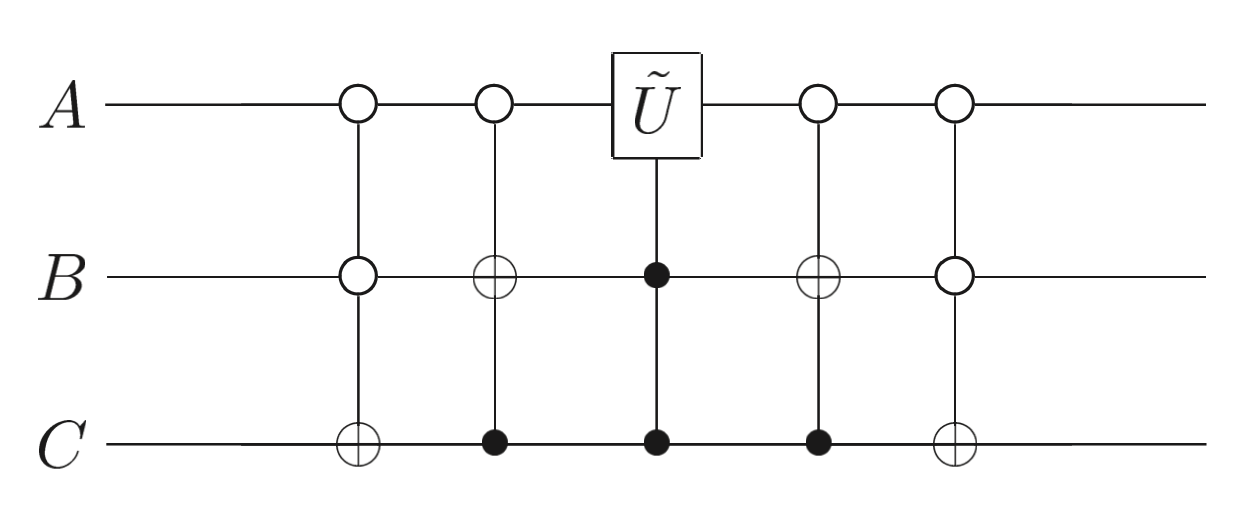
\includegraphics[width=0.5\linewidth]{U_hat_circuit.png}
    \caption{Circuit implementing the 2-level unitary $\tilde U$}
    \label{fig:enter-label}
\end{figure}

We can verify the equivalence of applying $U$ and the circuit on the previous examples:\\ 
\begin{center}
$\ket{000} \rightarrow \ket{001} \rightarrow \ket{011} \rightarrow U\ket{0} \cdot \ket{11} = (a\ket{0} + b\ket{1}) \cdot \ket{11} = a\ket{011} + b\ket{111} \rightarrow a\ket{001} + b\ket{111} \rightarrow a\ket{000} + b\ket{111} $ 
\end{center}
\begin{center}
$\ket{111}$: similar. 
\end{center}

What remains, in order to fully express the above quantum circuit in the desired shape, is to find a way to express the Toffoli gate ($CNOT$, conditioned on $2$ qubits), using single-qubit and $CNOT$ gates. This can be done, and below one can find the full circuit:\\
 \begin{figure}[h!]
     \centering
     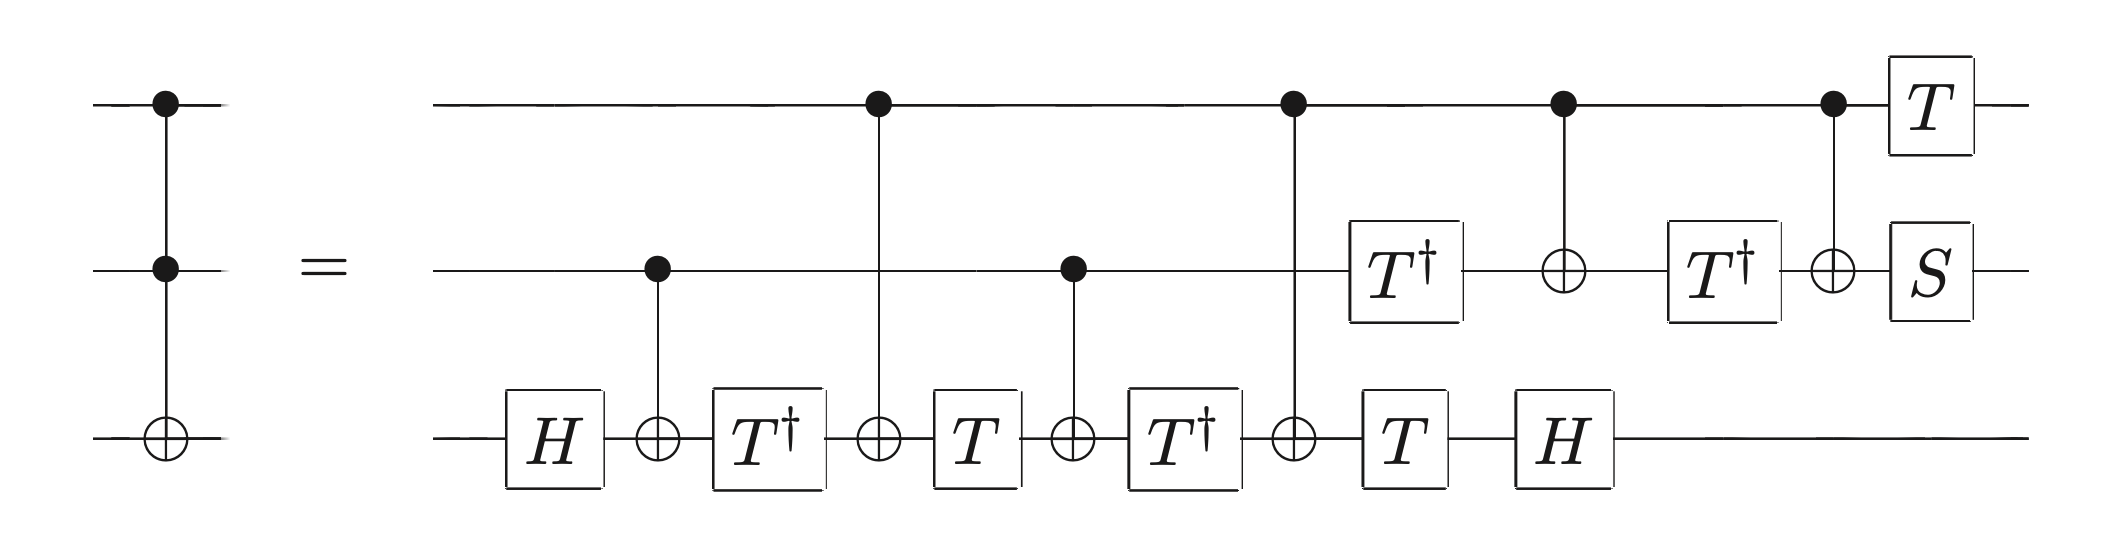
\includegraphics[width=0.9\linewidth]{Toffoli_sq_CNOT.png}
     \caption{Toffoli with single-qubit gates and $CNOT$s}
     \label{fig:enter-label}
 \end{figure}
}
\section{Step 3}
{Problem: Errors!
\begin{definition}
{
Error of using $V$ instead of $U$:\\
\[
E(U, V) = \max_{\lVert \psi \rVert = 1} \lVert (U - V) \ket{\psi} \rVert
\]
}
\end{definition}
\begin{proposition}
{
\[
\abs{P_U - P_V} \leq 2E(U,V),
\]
where $P_U$, $P_V$ are the probabilities of observing the same measurement outcome if $U$ or $V$ is applied.
}
\end{proposition}
\begin{proof}
{
Def. of $P_U$ + Cauchy-Schwarz inequality. 
}
\end{proof}
}

\begin{proposition}
{
$E(U_m  U_{m-1} \cdots U_1, V_m  V_{m-1} \cdots V_1) \leq \sum^{m}_{j=1} E(U_j, V_j)$
}
\end{proposition}
Moral: Errors add up at most linearly. \\

Lastly, after introducing the necessary concepts: universal approximation, 2 sets of gates.
\begin{enumerate}
    \item Standard set: $H$, $P$, $CNOT$, $\frac{\pi}{8}$.
    \item $H$, $P$, $CNOT$, Toffoli $\rightarrow$ more complicated!  
\end{enumerate}
Step 1: \\

$H$ and $\frac{\pi}{8}$ gates can approximate any single-qubit unitary up to an arbitrary accuracy. \\
\begin{property}
\begin{enumerate}
    \item $R_x(\theta) := e^{\frac{-i \theta X}{2}} = \cos{\frac{\theta}{2}} \cdot \mathds{1} - i  \sin{\frac{\theta}{2}} \cdot X$.\\
    \item $R_z(\theta) := e^{\frac{-i \theta Z}{2}} = \cos{\frac{\theta}{2}} \cdot \mathds{1} - i  \sin{\frac{\theta}{2}} \cdot Z=
        \begin{bmatrix}
            e^{\frac{-i \theta}{2}} & 0  \\
            0 & e^{\frac{i \theta}{2}} 
        \end{bmatrix}.$\\

    \item $T =
        \begin{bmatrix}
            1 & 0  \\
            0 & e^{\frac{i \pi}{4}}
        \end{bmatrix}
        = e^{\frac{i \pi}{8}} \cdot
            \begin{bmatrix}
                e^{\frac{-i \pi}{8}} & 0  \\
                0 & e^{\frac{i \pi}{8}}
            \end{bmatrix}
        = e^{\frac{i \pi}{8}} \cdot R_z(\frac{\pi}{4}) \equiv e^{\frac{-i \pi Z}{8}}$ \\
        \item $HTH \equiv e^{\frac{-i \pi X}{8}}$ \\
\end{enumerate}
\end{property}
Compose $T$, $HTH$:
\begin{align*}
e^{\frac{-i \pi Z}{8}} \cdot e^{\frac{-i \pi X}{8}} &= 
(\cos{\frac{\pi}{8}} \cdot \mathds{1} - i \sin{\frac{\pi}{8}} \cdot Z) \cdot (\cos{\frac{\pi}{8}} \cdot \mathds{1} - i \sin{\frac{\pi}{8}} \cdot X) \\
&= \cos^2{\frac{\pi}{8}} \cdot \mathds{1} - i (\cos{\frac{\pi}{8}} \cdot (X + Z) + \sin{\frac{\pi}{8} \cdot Y}) \cdot \sin{\frac{\pi}{8}} \\
\end{align*} \\
Rotation around $\overrightarrow{n}$ by $\theta$: 
$\hat{n} = (n_x, n_y, n_z)$, real unit vector in 3 dimensions. \\ \\
Now: $R_{\hat{n}}(\theta) = \cos(\frac{\theta}{2}) \cdot \mathds{1} - i \sin(\frac{\theta}{2})(n_x \cdot X + n_y \cdot Y + n_z \cdot Z)$.\\ 
\\
Hence, $T \circ HTH$ is a rotation:
\begin{itemize}
    \item about an axis $\hat{n} = (\cos(\frac{\pi}{8}), \sin(\frac{\pi}{8}), \cos(\frac{\pi}{8}))$;
    \item about an angle $\theta$ such that: $\cos(\frac{\theta}{2}) = \cos^2(\frac{\pi}{8})$;
\end{itemize}
Result: constructed $R_{\hat{n}}(\theta)$ with $H$ and $\frac{\pi}{8}$-gates.\\ \\
Step 2: \\

$\theta$ irrational $\Rightarrow$ since the set of irrational rotations is dense in the set of rotations, we can approximate rotation by any angle with $R_{\hat{n}}(\theta)$ up to arbitrary accuracy (will want up to $\epsilon / 3$). \\ \\
Step 3:\\

By Exercise 4.11 in Nielsen-Chuang: any unitary $U$ on a single qubit can be written as:
\begin{center}
    $U = R_{\hat{n}}(\beta) R_{\hat{m}}(\gamma) R_{\hat{n}}(\delta)$,
\end{center}
where $\hat{m}=(\cos(\frac{\pi}{8}), -\sin(\frac{\pi}{8}), \cos(\frac{\pi}{8}))$. (And $\hat{n} \nparallel \hat{m}$!) \\ \\
Also: $H R_{\hat{n}}(\alpha) H = R_{\hat{m}}(\alpha)$, since: \\ \\
\begin{align*}
H \cdot R_{\hat{n}}(\alpha) \cdot H &= H \cdot (\cos{\frac{\alpha}{2}} \cdot \mathds{1} - i \sin{\frac{\alpha}{2}}(n_x \cdot X + n_y \cdot Y + n_z \cdot Z)) H \\
&= H \cdot \cos{\frac{\alpha}{2}} \cdot \mathds{1} \cdot H - i \sin{\frac{\alpha}{2}}(n_x \cdot HXH + n_y \cdot HYH + n_z \cdot HZH) \\
&= H \cdot \cos{\frac{\alpha}{2}} \cdot \mathds{1} \cdot H - i \sin{\frac{\alpha}{2}}(n_x \cdot Z + n_y \cdot (-Y) + n_z \cdot X)\\
&= R_{\hat{m}}(\alpha)\\
\end{align*}
Then, for any $U$ on a single qubit:
\begin{enumerate}
    \item $U = R_{\hat{n}}(\beta) R_{\hat{m}}(\gamma) R_{\hat{n}}(\delta)$
    \item $R_{\hat{m}}(\gamma) = H R_{\hat{n}}(\gamma) H$
    \item $R_{\hat{n}}(\gamma) = (R_{\hat{n}}(\theta))^d$, $d$ some power.
\end{enumerate}

$R_{\hat{n}}(\beta) \xrightarrow{\epsilon / 3} R_{\hat{n}}(\theta))^{d_1}$, $R_{\hat{n}}(\delta) \xrightarrow{\epsilon / 3} R_{\hat{n}}(\theta))^{d_3}$. \\ \\
Combining this and applying 3) and 2) to the middle term $R_{\hat{m}}(\gamma)$, get:
\begin{center}
    $E(U, R_{\hat{n}}(\theta))^{d_1} \cdot HR_{\hat{n}}(\theta))^{d_2} H \cdot R_{\hat{n}}(\theta))^{d_3}) < \epsilon$,
\end{center}
by linear additivity of errors. \\
\subsection{Universality}

To summarize the above steps: 
\begin{itemize}
    \item any unitary = product of 2-level unitaries;
    \item any 2-level unitary = product of single qubit and $CNOT$ gates;
    \item any single qubit gate = product of $H$ and $\frac{\pi}{8}$ gates.
\end{itemize}
Thus, we can express any unitary, using only the $H$, $\frac{\pi}{8}$, $CNOT$ gates. \\

Lastly, some information on efficiency:
\begin{theorem} (Solovay-Kitaev)
    To approximate a circuit, containing $m$ CNOT's and single-qubit unitaries to an accuracy $\epsilon$: require $\mathcal{O}(m \log ^c \frac{m}{\epsilon})$ gates from the discrete set (which is likely to be accepted for all applications) ($c \approx 2$).
\end{theorem}
